\documentclass[border=10pt]{standalone}
\usepackage{tikz}
\usetikzlibrary{positioning, fit, arrows.meta, calc, backgrounds, shapes.geometric}

\begin{document}
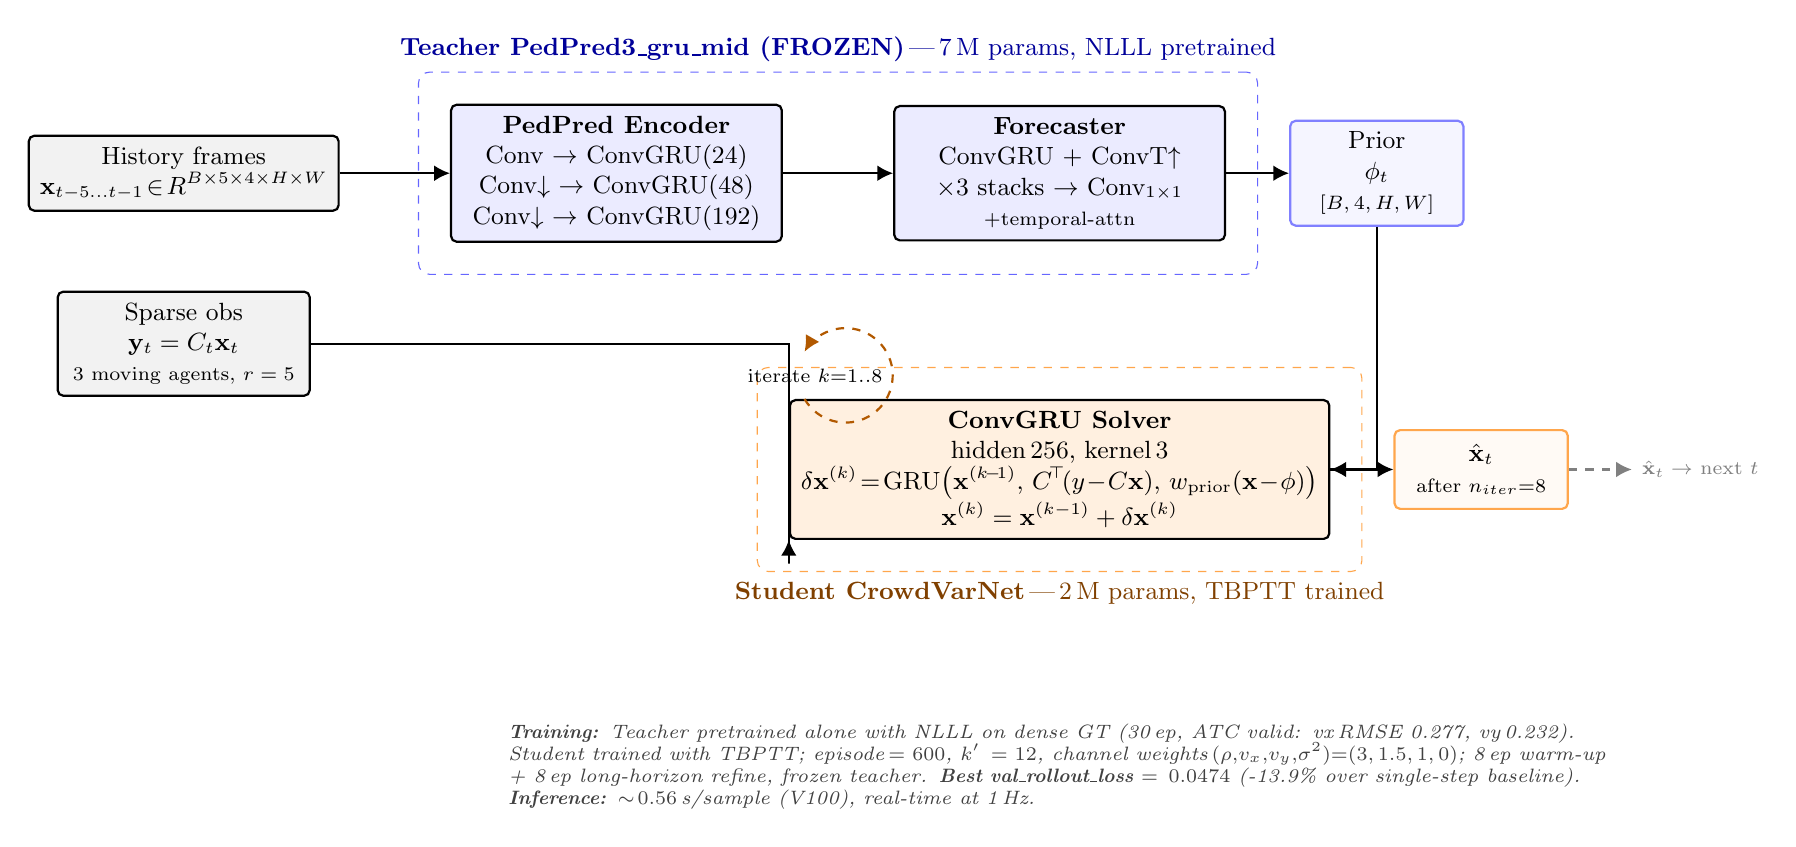
\begin{tikzpicture}[
  font=\small,
  node distance=10mm and 14mm,
  >={Latex[length=2mm,width=2mm]},
  block/.style={
    draw=black, thick, rounded corners=2pt,
    align=center, minimum height=10mm, inner sep=4pt
  },
  teacher/.style={block, fill=blue!8,  minimum width=42mm},
  solver/.style ={block, fill=orange!12, minimum width=42mm},
  io/.style     ={block, fill=gray!10, minimum width=32mm, minimum height=8mm},
  loop/.style   ={draw=orange!70!black, thick, dashed, rounded corners=4pt},
  lossnote/.style={font=\scriptsize\itshape, text=gray!50!black},
]

% ============ INPUTS ============
\node[io] (hist)
  {History frames\\$\mathbf{x}_{t-5\ldots t-1}\!\in\!\mathbb{R}^{B\times5\times4\times H\times W}$};

\node[io, below=of hist] (obs)
  {Sparse obs\\$\mathbf{y}_t = C_t \mathbf{x}_t$\\
   {\scriptsize 3 moving agents, $r=5$}};

% ============ TEACHER (FROZEN) ============
\node[teacher, right=of hist] (enc)
  {\textbf{PedPred Encoder}\\
   Conv {\small$\to$} ConvGRU(24)\\
   Conv$\downarrow$ {\small$\to$} ConvGRU(48)\\
   Conv$\downarrow$ {\small$\to$} ConvGRU(192)};

\node[teacher, right=of enc] (fore)
  {\textbf{Forecaster}\\
   ConvGRU + ConvT$\uparrow$\\
   $\times3$ stacks $\to$ Conv$_{1\times1}$\\
   {\scriptsize +temporal-attn}};

\node[block, fill=blue!4, draw=blue!50,
      right=8mm of fore, minimum width=22mm]
      (prior) {Prior\\$\boldsymbol{\phi}_t$\\{\scriptsize $[B,4,H,W]$}};

% Teacher box label (frozen)
\begin{scope}[on background layer]
\node[fit=(enc)(fore), draw=blue!60, dashed,
      rounded corners=4pt, inner sep=4mm,
      label={[blue!60!black]above:\small \textbf{Teacher PedPred3\_gru\_mid (FROZEN)}\,---\,7\,M params, NLLL pretrained}]
      (teacher_box) {};
\end{scope}

% ============ STUDENT SOLVER ============
\node[solver, below=20mm of fore] (solver)
  {\textbf{ConvGRU Solver}\\
   hidden\,256, kernel\,3\\
   $\delta\mathbf{x}^{(k)}\!=\!\mathrm{GRU}\bigl(\mathbf{x}^{(k\!-\!1)},\,
   C^{\!\top}\!(y\!-\!C\mathbf{x}),\,
   w_{\mathrm{prior}}(\mathbf{x}\!-\!\boldsymbol{\phi})\bigr)$\\
   $\mathbf{x}^{(k)} = \mathbf{x}^{(k-1)} + \delta\mathbf{x}^{(k)}$};

\node[block, fill=orange!4, draw=orange!70,
      right=8mm of solver, minimum width=22mm]
      (out) {$\hat{\mathbf{x}}_t$\\{\scriptsize after $n_{\text{iter}}{=}8$}};

% Student box label
\begin{scope}[on background layer]
\node[fit=(solver), draw=orange!70, dashed,
      rounded corners=4pt, inner sep=4mm,
      label={[orange!50!black]below:\small \textbf{Student CrowdVarNet}\,---\,2\,M params, TBPTT trained}]
      (student_box) {};
\end{scope}

% ============ EDGES ============
\draw[->, thick] (hist) -- (enc);
\draw[->, thick] (enc)  -- (fore);
\draw[->, thick] (fore) -- (prior);
\draw[->, thick] (prior.south) |- (solver.east);
\draw[->, thick] (obs.east)    -| ($(solver.south west)+(0,-3mm)$) -- (solver.south west);
\draw[->, thick] (solver) -- (out);

% Recurrence (k -> k-1)
\draw[loop, ->] (solver.north west) ++(2mm,0) arc (-150:150:6mm)
  node[midway, left, font=\scriptsize] {iterate $k{=}1..8$};

% Recurrence to next step (right of out, looping back)
\draw[->, gray, thick, dashed]
  (out.east) -- ++(8mm,0) node[right] {\scriptsize $\hat{\mathbf{x}}_t \to$ next $t$};

% ============ FOOTER (training annotations) ============
\node[lossnote, below=18mm of student_box.south, align=left, text width=140mm]
{
\textbf{Training:} Teacher pretrained alone with NLLL on dense GT (30\,ep, ATC valid: vx\,RMSE 0.277, vy\,0.232).
Student trained with TBPTT; episode\,$=600$, $k'\,=12$, channel weights\,$(\rho,\!v_x,\!v_y,\!\sigma^2){=}(3,1.5,1,0)$;
8\,ep warm-up + 8\,ep long-horizon refine, frozen teacher.
\textbf{Best val\_rollout\_loss} $= 0.0474$ (-13.9\% over single-step baseline).
\textbf{Inference:} $\sim\!0.56$\,s/sample (V100), real-time at 1\,Hz.
};

\end{tikzpicture}
\end{document}
